\chapter{Background}\label{chap:background}


Introduce the related state-of-the-art and background information in order to understand the method developed in the thesis. 

Automatic Machine learning which is described as the pipeline of steps, the repetitive steps are automated in order to save time and give more importance to other focus areas for an expert or to a end-user. In any application of machine learning one has to apply data pre-processing , feature extraction and feature engineering techniques to make data appropriate to be processed by any Machine learning algorithm. Once the data pre-processing to feature selection methods are applied, following is the selection of algorithms and its hyper-parameters based on the data. To gain a efficient model several optimization's has to be carried out. Automating these steps using certain probabilistic and stochastic methods such as Bayesian optimization and genetic programming gives us an advantage in gaining solutions to the problems faster and simpler. In context of aiding simple methods to solutions and improving the research on machine learning the term AutoML\cite{autoML} was coined. Under this several packages were developed some well know packages include Autosklearn\cite{autosklearn} TPOT\cite{tpot} AutoWeka\cite{autoweka-Thornton:2013:ACS:2487575.2487629} H2O AutoML. The interest of study in this thesis is on Autosklearn and TPOT since there methodologies are different and by evaluating these differences we would much gain more insight into Automatic machine learning.

\subsection{Machine Learning}

The term \blockquote{Machine learning} was coined in 1959 by Arthur Lee Samuel\footnote{\url{https://en.wikipedia.org/wiki/Arthur_Samuel}}. One of the first self-learning programs was developed by Arthur Samuel called Checkers-playing Program. The field of Artificial Intelligence had made its mark since then numerous research and development in the field of machine learning has led to where we are at the moment. One of the formal definitions of Machine learning(\textbf{ML}) was given by Tom Michael Mitchell\footnote{\url{https://en.wikipedia.org/wiki/Tom_M._Mitchell}} which states \blockquote{\textit{A computer program is said to learn from experience E with respect to some class of tasks T and performance measure P if its performance at tasks in T, as measured by P, improves with experience E}} from this simple definition we can have a surface understanding of how ML methodologies are developed and its applications to end-users. Humans have intelligence which enables them to think and arrive at an answer to a question. The derivation of the question and the process of tackling the possible solutions can be thought easily for a normal human brain, where as for a machine the process of handling and understanding the given tasks needs to be explicitly stated. The checkers-playing game\footnote{\url{https://en.wikipedia.org/wiki/Arthur_Samuel}} was built in such a way that every move was defined by a scoring function, for each move the outcome will be scored based on the number of pieces at the board at any position, each move was optimized in order to gain maximum chances of winning. Here the author instead of explicitly stating each move as an instruction devised a scoring function to optimize the next move reducing the computation resources without minimizing the outcome. In the early 21st century IBM developed a system called Watson\footnote{\url{https://en.wikipedia.org/wiki/Watson_(computer)}} which could answer questions posted in Natural Language, it also participated in a TV show where the participant needs to answer the questions 
asked by the host, Watson\footnote{\url{https://www.ibm.com/watson/about/}} won the contest against the current champions at that time. Compared to Arthur Lee Samuel's checkers game Watson is a highly complex AI system, still both follow the same fundamentals of AI that is there is no explicit programming before hand for the outcomes, the results are generated based on a variety of Optimization functions, Statistical approaches and Algorithms. 

In this day of Computer science ML has been developed to great heights with numerous algorithms to choose from. Industrial Research and Development aiding Machine learning it has become accessible to large extent of people even for those with no understanding of programming or ML domain. From the context of this thesis the methods from machine learning are described in the following sections

\subsubsection{Datasets in Machine learning}
Machine learning deals with data and there is lots of data being accumulated in this digital age every second, typical data used in machine learning involves series of samples from a entity for example a patient's hourly record on medicine intake, blood pressure and so on, these hourly sample constitute a data point/instance so for one day of the patient there will be 24 data points. Like these the data points gets accumulated over a period of time. Now these data points can be formatted in tabular format where each row is a sample and each column defines the values or the attributes such as blood pressure, age and so on. The tabular data which is now ready for machine learning process to begin. Just like these above explained data accumulation, there are many different domains of data available, basically in ML we deal with tabular form of data. A standard form of naming convention is followed for datasets, Each row is a sample/Instance each column is termed as features and at the last column contains a class or label which holds a value that is defined as the group or entity it belongs to, for example in a dataset of fruits every row contains information about the fruits properties, a label column at the end can be defined which will hold the name of the corresponding fruit the sample belongs. The datasets can nominal, numerical or categorical values,  further a training and testing set division is made in any machine learning process where training set may contain 80\% of the total dataset and rest 20\% is test set

\subsubsection{Types of machine learning}

\begin{figure}[!h]
    	\centering
    	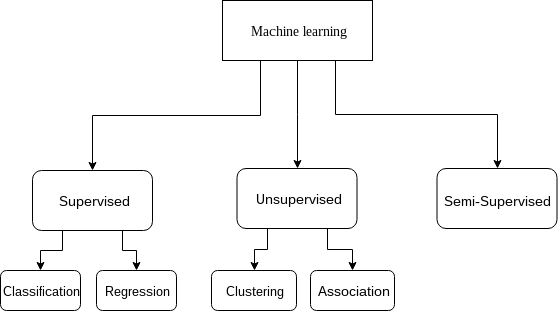
\includegraphics[width=0.9\linewidth]{thesis_template/images/machine_learning.png}
    	\caption{Machine learning Hierarchy}
    	\label{fig:machine_learning}
    \end{figure}
    
    
    \begin{figure}[!h]
    	\centering
    	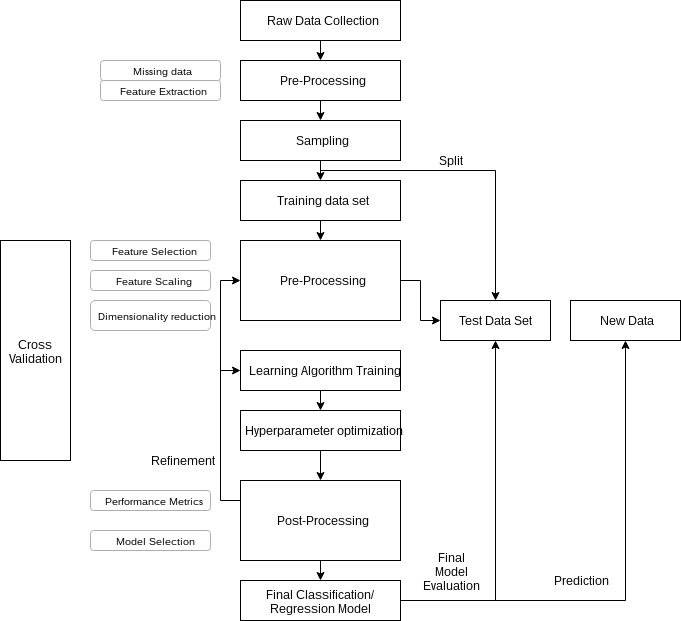
\includegraphics[width=1\linewidth]{thesis_template/images/machine_learning_workflow.png}
    	\caption{Machine learning Workflow}
    	\label{fig:machine_learning_workflow}
    \end{figure}
    
Machine learning involves certain types which depend on the task at hand, the task being the problem definition and the dataset, it has been divided into 3 main types that is Supervised, Unsupervised and Reinforcement learning. There are still other types of machine learning, here we will describe about the main three types.
\begin{itemize}
    \item Supervised Machine learning
     \begin{itemize}
        
         \item Supervised Machine learning deals with data samples which already has a label or target information available, for n samples of data, there should be n targets present to train any supervised machine learning algorithm. The main goal of supervised learning is to map a input that is a sample from the data to the output that is label or target. In this thesis we are dealing with supervised problems, there are two types in supervised learning
        
         \begin{itemize}
             \item Classification : This type deals with the data were the output is of a category or a class it belongs to for example fruit names apple or orange, and for a binary classification it can be high blood pressure or low blood pressure. The main hypothesis of classification is if a sample has probability of belonging to class or label from observation of trained data then that prediction would be  the outcome of the classifier 
             
             \item Regression : In Regression problems if the label or target contains a real valued number or continous value then the task is regression problem. examples of regression problem is when trying to predict the house prices based on the locality and the previous rates of the houses, regression is where the outcome would be a continuous quantity when compared to classification where it is a class or label
         \end{itemize}
         
     \end{itemize} 
     
     \item Unsupervised Machine learning
     
     \begin{itemize}
         \item Unsupervised learning deals with data samples were there is no label or target value present, In normal terms there is only Input but there is no output value available. The main focus of unsupervised learning is to learn the internal distribution of the data samples in order to gain more information on the data. Unsupervised learning is further divided into two types
         
         \begin{itemize}
             \item Clustering : Clustering as the name suggests it is a grouping of samples based on a particular attribute, for example grouping of customers based on there online purchase history
             \item Association : Association describes the rules from the data samples where certain rule suggest that a person who bought X can also buy Y
         \end{itemize}
     \end{itemize}
     
     \item Semi Supervised Machine learning
        \begin{itemize}
            \item This type of learning deals with datasets having very less labelled or target values available, semi supervised falls in between supervised and unsupervised were some of the data is only labelled. Real world problems are of semi supervised nature, labelled datasets are expensive and time consuming to produce and it involves experts in the field to produce such data.
        \end{itemize}
    
\end{itemize}

\subsection{Algorithms in Machine learning}
In scikit-learn\cite{scikit-learn} machine learning library there are several algorithms to work on, here in this section lets look into the basic algorithms of machine learning.

\begin{itemize}
    \item Naive Bayes 
    \begin{itemize}
        \item Naive Bayes algorithm is derived from Bayes rule which states that probability of an event based on prior knowledge  of conditions that might be related to the event\footnote{\url{https://en.wikipedia.org/wiki/Bayes\%27_theorem#Bayes'_rule}}. This is a supervised learning algorithm, from the Bayes rule it says there is no dependency between the features 
        \begin{equation}
            p(A|B) = \frac{p(B|A)  p(A)}{ p(B)} 
            \label{eqn:bayes_theorem}
        \end{equation}
        
        The equation \ref{eqn:bayes_theorem} is the mathematical representation of bayes theorem.
        Naive bayes algorithm has different varieties to it, some of them are Gaussian Naive bayes, Multinominal Naive Bayes, Bernoulli Naive Bayes each have there own assumptions on the given feature sets. These algorithms are favoured in text classification problems
      
    \end{itemize}
    
 \item Decesion Trees
    \begin{itemize}
            \item Decision Tree algorithm works with classification and regression problems that is it works with categorical and continuous variables. The algorithm tries to predict an outcome based on the feature rules obtained through learning. One of the advantages of Decision trees is that it can be visualized and easy to interpret and understand the workflow, fig \ref{fig:decision_tree} is a visualization of the decision tree conditional steps executed for iris dataset. Decision trees due to too many number of leaf nodes tend to over-fitting, care has to be taken in order to avoid over-fitting of the classifier.
            
            
        \begin{figure}[!h]
        	\centering
        	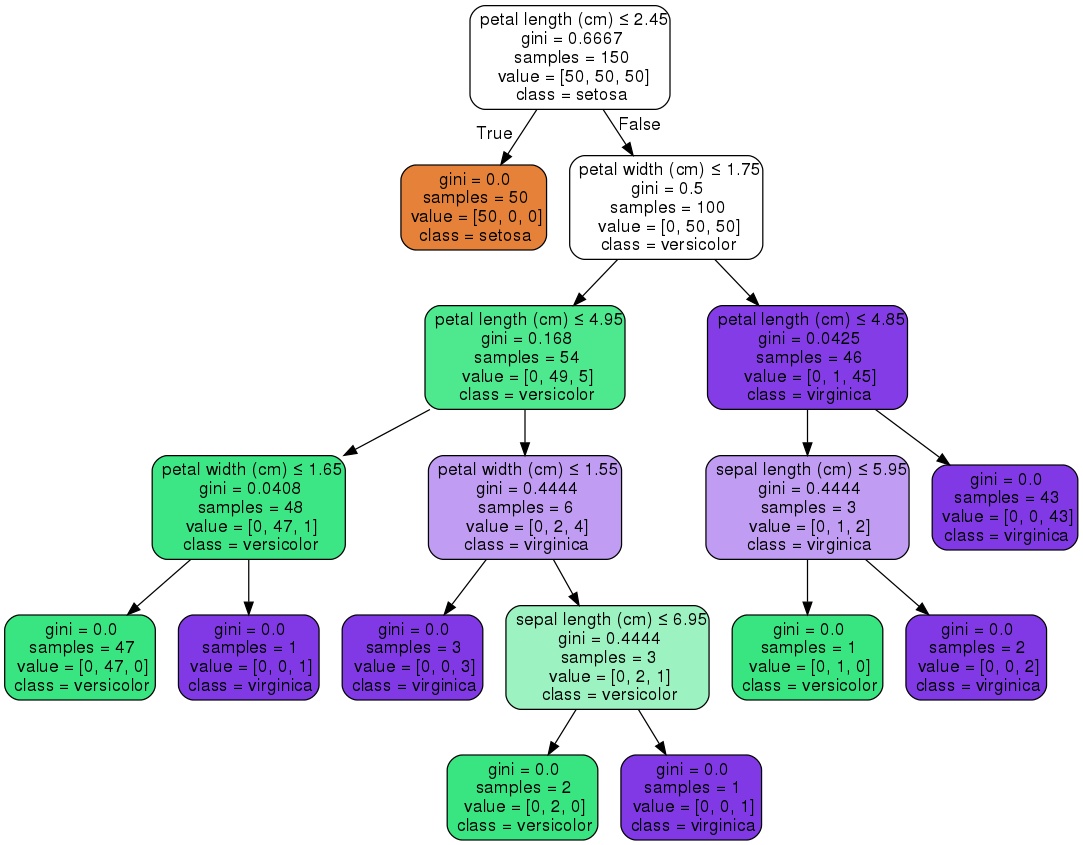
\includegraphics[width=0.8\linewidth]{thesis_template/images/decision_tree.png}
        	\caption{Decision trees Visualized}
        	\label{fig:decision_tree}
        	\captionsource{\url{https://scikit-learn.org/stable/modules/tree.html}}
        \end{figure}
        
    \end{itemize}
    
\item Support Vector Machine (SVM)
   \begin{itemize}
            \item SVM also works with classification and regression along with outlier detection problems, SVM's makes use of the kernal parameter in classifying the decision boundaries, for example if we have two features age and height of a person every feature will be a point drawn in 2 dimensional space where each point is 2D cordinate, these cordinates represent features, two lines will be drawn from the closet point in the 2D space and then between these lines a classifier boundary line will be drawn bisecting the two feature space which is divided by the other two lines drawn at first, this classifier line is the next decision maker when there is new feature to classify against the 2D space of the features, fig \ref{fig:svm} describes the process of finding the decision boundary between the two features plotted. The equation \ref{eqn:svm_decision} is the function used to calculate the decision line.
            
            \begin{equation}
                \operatorname{sgn}(\sum_{i=1}^n y_i \alpha_i K(x_i, x) + \rho)
                \label{eqn:svm_decision}
            \end{equation}
            
            
            \begin{figure}[!h]
        	\centering
        	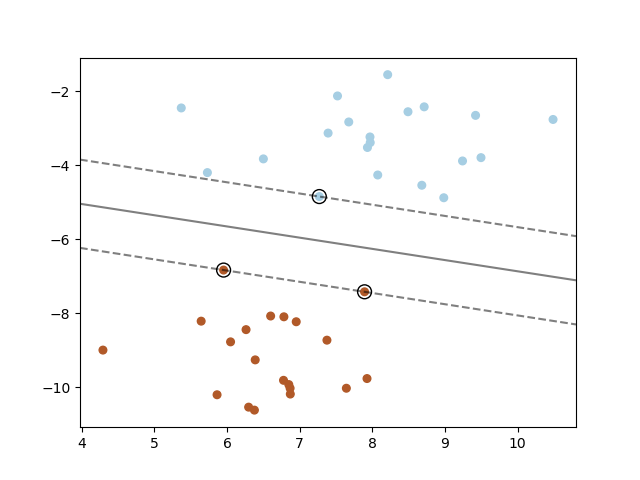
\includegraphics[width=0.6\linewidth]{thesis_template/images/svm.png}
        	\caption{Support vector machine}
        	\label{fig:svm}
        	\captionsource{\url{https://scikit-learn.org/stable/modules/svm.html}}
            \end{figure}
            
    \end{itemize}
    
\item Random Forest
\begin{itemize}
    \item \cite{random-forest}Random forest supports classification and regression, this algorithm is a type of ensemble algorithm where multiple samples are taken at a time and models are created for each of them, while predicting the output the mean from all the models is considered to give a optimal output for the input, there might be bias due to samples drawn randomly but since they average out the prediction at the end the variance decreases. Random forest algorithm is one of the most popular algorithms used.
\end{itemize}

\item Linear Regression
\begin{itemize}
    \item There are two types of Linear regression one is Simple linear regression and Multiple Linear regression.
    Linear regression is used to find the relation between 2 continuous variables one is the actual input and other one is the predictor variable, in the fig \ref{fig:linreg} the blue inidicates the linear regression line were its drawn between the samples of data, the line is best fit when its drawn with minimal error that is minimal distance from samples , once the line is drawn the new input variable has to be predicted with minimal error, that is less than or equal to minimum error from the line drawn. In the equation \ref{eqn:linreg} the values of w\_0 and w_1 should be chosen such that they minimize the error. formally stating Linear regression fits a linear model with variables such that the error margin is less and such that it best fits the data.
    
    \begin{equation}
        \hat{y}(w, x) = w_0 + w_1 x_1 + ... + w_p x_p
        \label{eqn:linreg}
    \end{equation}
    
    \begin{figure}[!h]
        	\centering
        	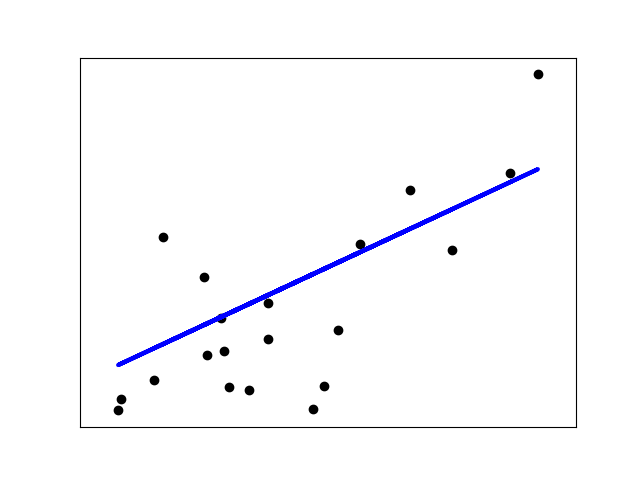
\includegraphics[width=0.6\linewidth]{thesis_template/images/linreg.png}
        	\caption{Linear Regression}
        	\label{fig:linreg}
        	\captionsource{\url{https://scikit-learn.org/stable/modules/linear_model.html}}
            \end{figure}
            
\end{itemize}
\end{itemize}

\subsection{Feature engineering methods in Machine learning}

\subsection{Ensemble Methods}
The technique of ensemble methods is to combine different models together to have a better estimate of the outcome and to improve over a single model, each combined model is with different algorithm and different feature engineering techniques combined, there are two types of ensemble methods
\begin{itemize}
    \item Bagging methods 
    \begin{itemize}
        \item In averaging method, all the models which are combined, the predictions of each model will be averaged for a single prediction, here due to this process the variance is reduced and its better than the single model's prediction
    \end{itemize}
    
    \item Boosting methods
    \begin{itemize}
        \item In this technique its contrary to Bagging, several models will be built and each  tries to reduce the variance or the bias making it a power full ensemble by combining weak models together to form a better model
    \end{itemize}
\end{itemize}

Ensemble methods are very powerfull when combined with series of different feature encoders and transformers when required with a single estimator at the end, these type of combination can account for the imbalance in predictions and provide a more optimal prediction score over a single model. Most commonly used estimators with ensembles are Random forests, Gradient boosting, ExtraTrees. This technique is used in Autosklearn for construction of ensemble from different models which are trained during the execution

\subsection{Machine learning pipeline}
Machine learning pipeline is a simple method which consists of series of Transformers and at the end a estimator, pipeline is used basically to combine series of operations into one method and to set different parameters during execution using cross-validation or repeated learning, the starting steps of the pipeline should be transformers which must implement transform and fit methods and last step should be the algorithm which needs to only implement fit method. This is a simple utilty from sklearn\cite{scikit-learn} used to sequence the steps in order of a typical Machine learning workflow


\subsection{Range of evaluation metrics}

There are a range of metrics to choose from when evaluating a machine learning model, evalaution of a model is necessary in order to obtain a better prediction out of it and to asses how good the model is performing. The selection of metrics depends on the estimator type, there are different kind of metrics for classification and regression problems
\begin{itemize}
    \item Classification Metrics
    \begin{itemize}
        \item Classification accuracy : This is the most common metric used for classification problems, it is defined has the no of correct predictions divided by the total number of predictions made, one drawback of this metric is it does not take into account the sample distributions, if there is a imbalance of class variables accuracy tends to bias towards the majority class.
        
        \begin{equation}
            \displaystyle{Accuracy} = \frac{\displaystyle{No of correct predictions}}{Total no of predictions made}
        \end{equation}
        
        \item Confusion Matrix : Its a matrix output of the model's performance, there are 4 main variables in confusion matrix. if there is classification problem or tumor YES or tumor NO
        \begin{itemize}
            \item True Positives : The model predicted YES and the actual value is also YES
            
            \item True Negatives : The model predicted NO and the actual value is also NO
            
            \item False Positive : The model predicted NO and the actual value is YES
            
            \item False Negative : The model predicted NO and the actual value is YES
        \end{itemize}
        
        \item Area Under Curve : Mainly used for binary classification problems, there are two basic terms under AUC 
        \begin{itemize}
            \item True Positive Rate : Its defined as in this equation \ref{eqn:tpr}, also known as Sensitivity 
            \begin{equation}
                \displaystyle{True Positive Rate} = \frac{\displaystyle{TP}}{\displaystyle{FP + TP}}
                \label{eqn:tpr}
            \end{equation}
            
            \item False Positive Rate : Its defined as in this equation \ref{eqn:fpr}, also known as Specificity
            \begin{equation}
                \displaystyle{False Positive Rate} = \frac{\displaystyle{FP}}{\displaystyle{FP + TN}}
                \label{eqn:fpr}
            \end{equation}
        \end{itemize}
       
        \begin{figure}[!h]
        	\centering
        	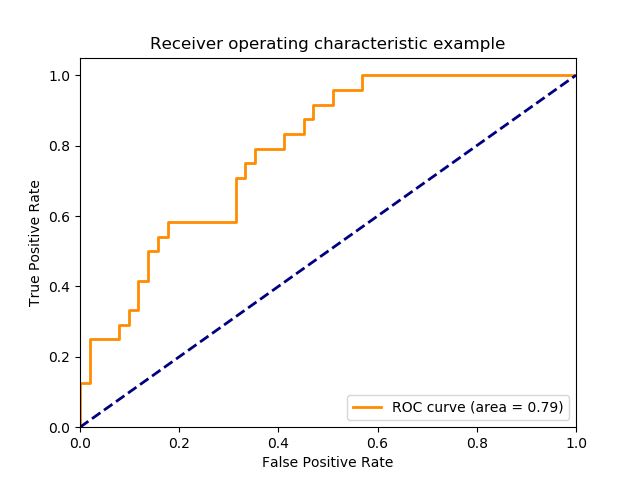
\includegraphics[width=0.6\linewidth]{thesis_template/images/auc.png}
        	\caption{AUC curve}
        	\label{fig:auc}
        	\captionsource{\url{https://scikit-learn.org/stable/auto_examples/model_selection/plot_roc.html#sphx-glr-auto-examples-model-selection-plot-roc-py}}
            \end{figure}
        
        
        Auc has range of 0,1, tpr and fpr have in range of 0.00, 1.00 when these values are plotted in a graph the line under ROC is AUC, higher the value of AUC better the performance of the model
        
        \item F1-score : It is the balance between precision and recall, by calculating the harmonic mean between them\footnote{\url{https://towardsdatascience.com/metrics-to-evaluate-your-machine-learning-algorithm-f10ba6e38234}}. It can also tell how precise a classifier is and how flexible the prediction values, the equation \ref{eqn:f1score} defines the f1-score
        
        \begin{equation}
            F1 = 2 * \frac{1}{\frac{1}{precision} + \frac{1}{recall}}
            \label{eqn:f1score}
        \end{equation}
        
        Precision is defined as \ref{eqn:pr}
         \begin{equation}
            Precision = \frac{TP}{TP + FP}
            \label{eqn:pr}
        \end{equation}
        
        Recall is defined as \ref{eqn:r}
         \begin{equation}
            Recall = \frac{TP}{TP + FN}
            \label{eqn:r}
        \end{equation}
        
    \end{itemize}
    
    
    \item Regression Metrics
    \begin{itemize}
        \item Mean squared error : MSE takes the average of the square of the difference between the original values and the predicted values. Commonly used for regression tasks, the equation \ref{eqn:mse} defines the function of MSE
        
        \begin{equation}
            \text{MSE}(y, \hat{y}) = \frac{1}{n_\text{samples}} \sum_{i=0}^{n_\text{samples} - 1} (y_i - \hat{y}_i)^2.
            \label{eqn:mse}
        \end{equation}
    \end{itemize}
    
    These metrics are the common performance metrics used in ML practice, still there are other methods such as Statistical significance tests and validation , learning curves which can emphasize the model behaviour in much more detail.
    
\end{itemize}



\subsection{Bayesian Optimization}

Bayesian optimization is a method of optimizing a function which is very time consuming to produce an outcome. In our case tuning of hyper-parameters for an algorithm which is demonstrated in Autosklearn\cite{autosklearn}. In simple terms a function \textit{f(x)} has to be optimized within a number of steps, having the number of steps as a threshold is the budget or the cost \textit{c}. Bayesian optimization will take assumptions about the function \textit{f(x)} and then updates those previous assumptions with the samples drawn out from the function \textit{f(x)}, this will provide a an estimate on where to evaluate next in the upcoming iterations i.e in which part of the search space does the important hyper-parameters has to be searched. This will minimize the number of steps to reach a optimal solution.